%! TEX root = thesis

\chapter{Free-energy landscapes}

\section{Introduction}

Consider a system of $N$ classical particles in $d$ dimensions.  If the position of the $i$th particle is given by the position vector $\bm{r}_{i} \in \mathbb{R}^{d}$, then the entire configuration of the system can be fully described at any moment using a configuration vector $\bm{r} \in \mathscr{R} \subseteq \mathbb{R}^{Nd}$ defined by $\bm{r} = (\bm{r}_{1}, \bm{r}_{2}, \ldots, \bm{r}_{N})$.
  Here $\mathscr{R}$ is the ambient space.%
  \footnote{Many authors~\cite{littlejohn1997,lelievre2010} call $\mathscr{R}$ as the configuration space.  However, when constraints are imposed on the system, the actual configuration space is usually a lower-dimensional subset of $\mathscr{R}$.  To make this distinction, we will call $\mathscr{R}$ as the ambient space.}
Corresponding to $\bm{r}$ we define a momentum vector $\bm{p} = (\bm{p}_{1}, \bm{p}_{2}, \ldots, \bm{p}_{N})$, where $\bm{p}_{i}$ is the momentum of the $i$th particle.
Since there is no apriori reason for the momenta to be bounded, $\bm{p} \in \mathbb{R}^{n}$.
The microscopic state of the system at a given moment is described by the position-momentum pair $(\bm{r}, \bm{p}) \in T^{*}\mathscr{R}$, where $T^{*}\mathscr{R}$ is the cotangent bundle.
The expectation value of a macroscopic observable $\hat{\xi}$ is
%
\begin{equation}
  \braket{\hat{\xi}} = \int_{T^{*}\mathscr{R}} \dd\mu(\bm{r}, \bm{p})\, \hat{\xi}(\bm{r}, \bm{p}).
\end{equation}

\subsection{Marginal probability densities}

The marginal probability density $\mathscr{P}(\xi)$ in terms of $\xi \in \mathbb{R}^{m}$ with $m \geq 1$ defined as%
\footnote{This equation has been called the ``random variable transformation theorem''~\cite{gillespie1983} and can be used to prove a number of useful results in elementary probability theory; also see Ref.~\cite[Section~I.5]{kampen2007}.}
%
\begin{equation}
  \mathscr{P}(\xi) = \int \dd{\bm{r}}\, \delta[\hat{\xi}(\bm{r}) - \xi] \mathscr{P}(\bm{r}).
  \label{c03:eq:probtrans}
\end{equation}
%
To show that the above equation gives the correct marginal density, we first note that the average $\braket{\phi}$ of an observable $\phi \equiv \phi(\xi) = \phi[\hat{\xi}(\bm{r})]$ that only depends on the transformed variable $\xi$ can be computed using either the transformed density $\mathscr{P}(\xi)$ or the original density $\mathscr{P}(\bm{r})$, i.e.,
%
\begin{equation}
  \braket{\phi} = \int \dd{\tilde{\xi}}\, \phi(\tilde{\xi}) \mathscr{P}(\tilde{\xi}) = \int \dd{\bm{r}}\, \phi[\hat{\xi}(\bm{r})] \mathscr{P}(\bm{r}).
\end{equation}
%
Taking $\phi(\tilde{\xi}) = \delta(\tilde{\xi} - \xi)$ yields
%
\begin{equation}
  \int \dd{\tilde{\xi}}\, \delta(\tilde{\xi} - \xi) \mathscr{P}(\tilde{\xi}) = \mathscr{P}(\xi) = \int \dd{\bm{r}}\, \delta[\hat{\xi}(\bm{r}) - \xi] \mathscr{P}(\bm{r}).
\end{equation}

\subsubsection{Free energy of a stiff rotor}

Consider a rotor of unit natural length in two dimensions centered around the origin with a rotationally symmetric potential energy\footnote{We could have also chosen the more conventional energy function $U(x, y) = \kappa(\sqrt{x^2 + y^2} - 1)^2$, but that makes the integrals that follow difficult to evaluate exactly.  One can still asymptotically evaluate it by Taylor expanding $U(x, y)$ around the saddle point $y = \sqrt{1 - x^2}$ to $\mathcal{O}(y^4)$.} $U(x, y) = \kappa(x^2 + y^2 - 1)^2$, with $\kappa$ being a ``spring constant'' to set the units.
This potential energy function achieves its minimum on the unit circle $x^2 + y^2 = 1$, which is our constraint level set $\Omega$.
Choosing the $x$ coordinate of the rotor as our \ac{cv}, we have the \ac{cv} map $\hat{x}: (x,y) \mapsto x$, and the \ac{pdf} of the \ac{cv} is
%
\begin{equation}
  \begin{aligned}
    \mathcal{P}_{\hat{x}}(x) &= \int_{-\infty}^{\infty} \dd{y}\, \exp\left[-\beta\kappa(x^2 + y^2 - 1)^2\right]\\
                             &= (2\beta\kappa)^{-1/4}\exp\left[-\beta\kappa(x^2 - 1)^2\right]\,\int_{0}^{\infty} \dd{t}\,t^{-1/2}\exp\left[-\tfrac{1}{2}t^2 - \sqrt{2\beta\kappa}(x^2 - 1)t\right]\\
                             &= \sqrt{\pi}(2\beta\kappa)^{-1/4}\exp\left[-\tfrac{1}{2}\beta\kappa(x^2 - 1)^2\right]D_{-1/2}\left[\sqrt{2\beta\kappa}(x^2 - 1)\right]\,,
  \end{aligned}
\end{equation}
%
where $D_{-1/2}[\,\cdot\,]$ is the parabolic cylinder function%
\footnote{We can also write $\mathcal{P}_{\hat{x}}(x)$ in terms of the modified Bessel function of the second kind $K_{1/4}(\,\cdot\,)$ after making use of the relation $D_{-1/2}(z) = \sqrt{z/(2\pi)}K_{1/4}(z^2/4)$ \cite[Eq.~12.7.10]{olver2010}.
This is the result that \ac{cas} often produce.} \cite[Eq.~12.5.1]{olver2010}.
Using $\mathcal{P}_{\hat{x}}(x)$ we find the free-energy difference to be
\begin{equation}
\begin{aligned}\label{eq:rotor_exact_a}
  \mathcal{A}_{\hat{x}}(x) - \mathcal{A}_{\hat{x}}(0) &= -\beta^{-1}\log{\mathcal{P}_{\hat{x}}(x)} +\beta^{-1}\log{\mathcal{P}_{\hat{x}}(0)}\\
                                                      &= \tfrac{1}{2}\kappa(x^4 - 2x^2) - \beta^{-1}\log\left\{\frac{D_{-1/2}\left[\sqrt{2\beta\kappa}(x^2-1)\right]}{D_{-1/2}\left(-\sqrt{2\beta\kappa}\right)}\right\}\,.
\end{aligned}
\end{equation}
But what if one evaluates the integral in Eq.~XXX asymptotically for large $\beta$ using Laplace's method?
Two (standard) parameterizations in $x$ that cover the entire circle $S^1$ are
\begin{equation}
  \psi_{\pm}(x) = (x, \pm\sqrt{1 - x^2})\,,
\end{equation}
and the corresponding induced metrics are
\begin{equation}
  |\det g_{\pm}(x)| = (1-x^2)^{-1}\,.
\end{equation}
It is clear that there is a coordinate singularity at $x = \pm 1$ where $|\det g_{\pm}(x)|$ diverges.
Meanwhile, the dynamical matrix is
\begin{equation}
  \hess U(x, \pm\sqrt{1-x^2}) = 8\kappa
  \begin{pmatrix}
    x^2 & \pm x\sqrt{1-x^2}\\
    \pm x\sqrt{1-x^2} & 1-x^2
  \end{pmatrix}\,,
\end{equation}
which has only one nonzero eigenvalue, $8\kappa$.
Making use of Eq.~XXX, we get the asymptotic \ac{pdf} (which is a rescaled $\beta$ PDF for parameters $(1/2, 1/2)$.)
\begin{equation}
  \mathcal{P}_{\hat{x}}(x) = \sqrt{\frac{\pi}{\beta\kappa(1-x^2)}} + \mathcal{O}(\beta^{-3/2})\,,
\end{equation}
which leads to
\begin{equation}\label{eq:rotor_asy_a}
  \mathcal{A}_{\hat{x}}(x) - \mathcal{A}_{\hat{x}}(0) = \beta^{-1}\log\sqrt{1-x^2}\,.
\end{equation}
\begin{figure}
  \begin{center}
    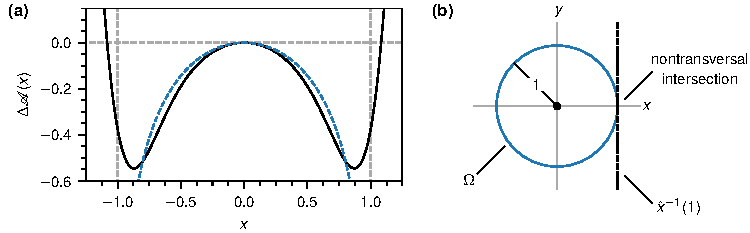
\includegraphics[scale=1.0]{rotor.pdf}
  \end{center}
  \caption{
    Free-energy difference $\mathcal{A}_{\hat{x}}(x) - \mathcal{A}_{\hat{x}}(0)$ of the stiff rotor at inverse temperature $\beta = 100$, from numerical simulations (black solid line), asymptotic expression (Eq.~\ref{eq:rotor_asy_a}; blue dashed line), and exact expression (Eq.~\ref{eq:rotor_exact_a}; red dashed line).
    Note how the asymptotic expression has a logarithmic divergence at $x = \pm 1$.
    Also note that the free-energy minimum is \emph{not} at $x = \pm 1$ as one might guess (or how the asymptotic expression suggests).
  }
  \label{fig:rotor}
\end{figure}

\section{Hard vs. soft constraints}

Trimer discussed in Refs.~\cite{kampen1981,kampen1984} (and also in Refs.~\cite[Section 15.1]{frenkel2001} and \cite{walter2011})

\section{CV under a transformation that is not smooth}

The free energy difference becomes
%
\begin{equation}
  \Delta\free{\xi} = -\beta^{-1}\log\left[\frac{\sqrt{\pi}\left(\abs{\cos\xi'} + \abs{\sin\xi'}\right)}{2 + \sqrt{X}D_{-1/2}(0)\left(1 + Y\right)}\right]
\end{equation}
\begin{equation}
  \begin{aligned}
    \Delta\free{\xi} &= \beta^{-1}\log\left[2 + \sqrt{X}D_{-1/2}(0)\left(1 + Y\right)\right] \\
                     &\qquad -\beta^{-1}\log\Big\{2\abs{\cos\xi'}^{-1} + \sqrt{X}\big[\exp(-X^{2}\xi'^{4})D_{-1/2}(-2X\xi'^{2})\\
                     & \phantom{\qquad-\beta^{-1}\log\Big\{2\abs{\cos\xi'}^{-1} + \sqrt{X}\big[}
                 \quad+Y\exp(-X^{2}Y^{2}\xi'^{4})D_{-1/2}(-2XY\xi'^{2})\big]\Big\}   \end{aligned}
\end{equation}
%
Here $\xi' = \pi\xi/4$.

\subsubsection{Cone-plane intersection}

A singularity is formed at the origin when a cone $z^2 = x^2 + y^2$ intersects with the $yz$ plane.
However, there's no lowering of the free energy since the intersection isn't a nontransversal intersection.
The only plane tangent to the $yz$ plane is the $yz$ plane itself, which is not tangential to the cone at the origin.
One might object that the cone itself ceases to be a manifold at the origin.
However, one can always ``file off'' the tip of the cone and make it infinitesimally smooth like a physicist would do.
This would still produce no lowering of the free energy.
